\documentclass{article}
\usepackage[utf8]{inputenc}
\usepackage{graphicx}
\graphicspath{ {./images/} }

\title{Microsoft Research Sentence Completion Challenge}
\author{J Bali (219057)}
\date{2022\\ 
\\
2392 words}



\begin{document}


\maketitle

\begin{abstract}
The Microsoft Research Sentence Completion Challenge requires a system to  be able to predict which is the most likely word (from a set of 5 possibilities) to complete a sentence. In this paper we discuss our experiments to complete this challenge. We start with a very simple random baseline and compare the accuracy of this system to that of unigram and bigram models. We then discuss the construction of trigram and quadrigram models, and how the accuracy of these models changes as we increase the size of our context window. Lastly, we compare the accuracy of these models to that of the BERT pre-trained model, which we find to be much more accurate. To conclude, we discuss how the accuracy of our system could be increased with more time for research and experimentation.
\end{abstract}

\newpage

\section{Introduction}
Constructed by Microsoft Research in 2011, the Sentence Completion Challenge (SCC) is a data set consisting of 1040 randomly selected sentences from Conan Doyle's Sherlock Holmes novels, each with a single word removed and replaced with a blank space token. Each sentence in the set is accompanied by 5 options for this masked word, one of which is the original word. The other 4 words are possible alternatives that were automatically generated using an n-gram language model trained on 540 19th century novels. (Zweig and Burges, 2011) The MRSCC data set exists for authors of semantic models to measure and compare how well their systems work, so we will use it to evaluate a selection of techniques.

\section{Generating a Baseline}
As a fundamental baseline, we allowed a system to randomly select answers to each of the questions in the data set. This random system (which will act as our most simple baseline) achieved an accuracy of 20\% as expected. We can deem a system functional if it is more accurate than the random baseline.

To make a more meaningful baseline, we constructed two very simple n-gram models. First, a unigram, which does not check for context, and just returns the most common word of the given options; and second a bigram, which checks one word to the left for context to generate a probability for each of the target words.

The process of creating an n-gram is very simple. The system searches through each word in the corpus, constructing a dictionary of contexts and building up probabilities for proceeding words. A unigram does not search for this context, so just finds a probability as the number of occurances of a given word, divided by the total number of words in the corpus. A bigram looks one word to the left for context, so creates a dictionary based on this context. In the example phrase "the cat sat on the mat," a bigram would find the word "the" and see that it is proceeded by "cat" and "mat" in 2 different places. The dictionary for the context word "the" would build up probabilities for these two words, in this case giving them equal probability. As more data is given to the n-gram generator, the probabilities would change. After searching through all 522 novels in our training corpus (our dataset contains 522 instead of the 540 the Microsoft Research team used due to copyright reasons), the word "the" will have a lot more than just the two potential follow-up words, and the probabilities will be a lot more complex.

The unigram we constructed has an accuracy of 24.71\%, making it slightly better than the random baseline. The reason it is better is because it looks at the likelihood of words appearing. In some of the questions in the challenge, the imposter words are extremely uncommon, so they will be ignored by the unigram. The unigram has no context, so it is still not very accurate. The bigram is slightly more accurate, at 26.45\% accuracy. With the single word of context, the bigram is slightly more informed in its predictions. The bigram's probabilities are split into contexts, so the chances of it making mistakes is lower, but due to the very small context it will still be quite inaccurate.

\section{Further N-Gram Models}
With our baselines set, we can move on to creating some more accurate solutions. Since we have an n-gram system already constructed, we decided to start our research by extending the n-gram system to search for more context in the form of a trigram and quadrigram.

\subsection{Construction}
The construction of higher value n-grams is not much different to the construction of the bigram. In a trigram, we create nested dictionaries, such that $trigram[context1]$ gives us another dictionary to search for a second context word. The dictionary returned by this second context word check can then be checked for the target word to find its probability. Some of the questions in the challenge have very generic context phrases. Before the masked token, question 61 has the context "I have ..." and question 71 has the context "Then he ...". Both of these questions are so generic in their context, and have so many possible follow-up tokens that it is infeasible for a system to have a high accuracy when using smaller n-grams.

The quadrigram we are constructing then adds a further layer on top of the trigram, allowing a 3rd context word to be added. This further narrows the options for target words for a given context, potentially increasing the accuracy of the system. There is the possibility that some of the combinations of context phrases and target words will not appear in the high n-grams, which will in turn decrease the accuracy again. The problems that our n-grams are not able to find a possible solution to will have a randomly selected solution added instead. 

\begin{figure}[h]
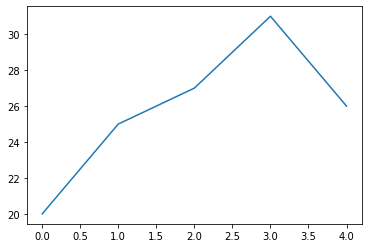
\includegraphics[width=6.5cm]{graph1.png}
\centering
\caption{A graph showing the change in accuracy as the value of n increases.}
\end{figure}

\subsection{Analysis}
We recorded the accuracy of each of our n-grams to find any trend in the change in accuracy as n increased. As seen in figure 1 (at the end of the previous page), the accuracy of the system increases from the baselines (n=0 for the random system and n=1 for the unigram), but only to a point. The accuracy of the system peaks at 31.58\% with the trigram, decreasing afterwards, with the accuracy of the quadrigram being lower than that of the bigram. This shows that n-grams as a system are not infallible and eventually drop off as the number of combinations decreases. It's important to find the perfect balance between having enough combinations to get meaningful results, and not being too restrictive as to lose combinations.

\begin{figure}[h]
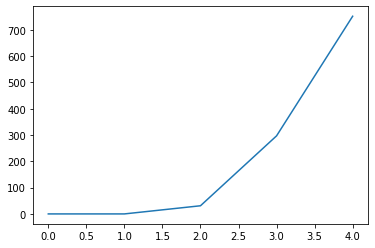
\includegraphics[width=6.5cm]{graph2.png}
\centering
\caption{A graph showing the number of times the correct target was left unfound for each value of n.}
\end{figure}

This second graph shows the number of problems in the SCC that the n-gram was unable to find a possible solution to, either because the context phrase or the target word didn't exist in its memory. It can be seen that even the bigram starts to lose combinations. The bigram finds this issue occurs 31 times, though this is most likely due to the context phrases containing proper nouns or obscure words - Question 921, for example, has the context phrase "Colonel Lysander Stark ..." which, as a proper noun, will not have occurred in the training data. The number of errors increases exponentially, and the quadrigram was unable to find a solution 752 times. As a test to find what the bottleneck in the n-gram system is, we decided to test the accuracy of the quadrigram, given only the problems it was able to find a solution to. By looking only at the 288 problems the quadrigram was able to find a solution to, we got an accuracy of 45.50\%, showing that the inability to find possible solutions was a large bottleneck in the system.

Question 618 has the context phrase "a patriarch among ..." which is a phrase that is very unlikely to appear in speech. A bigram may have found a potential answer with this context phrase, as "among" is a fairly common word, but the quadrigram, which searches a larger context window, will be less likely to find answers with less-common words and word combinations.

This downside may be resolved by stacking the n-gram models together. The accuracy of smaller n-grams is lower than the larger ones, but the number of unfound solutions is also lower. It is possible that a problem unfound by the quadrigram may be found by the trigram, and the accuracy of the trigram is still higher than that of the baseline. By continuing to check through incrementally smaller n-grams until a solution is found, we may be able to find a more accurate solution. The initial paper released by Microsoft Research suggested this solution as a more sophisticated baseline, finding a 34\% accuracy for the itterative n-gram system - 2.42\% higher than our simple trigram. (Zweig and Bruges, 2011) 

\subsection{Neural N-Gram Variant}
N-grams are particularly good for text generation, but they have a lot of downsides when it comes to finding masked words in a given sentence due to their small context size. A solution to this is the use of a fully-recurrent (Hopfield-style) neural network. A hopfield network is a circular neural network that has a node for every unique word in a corpus (Hopfield, 1982). The weights of the connections between the nodes would be incremented symmetrically with each co-occurrence of a word in a given training sentence. When the full training corpus has been searched through, the sums would need to be normalised into the probability of two words co-occurring in a sentence. Functionally, this is a more advanced version of an n-gram model, as it just checks a context window and finds the most likely outcome, based on the average probability of co-occurance. The advantage of using this novel system would be an increase in the context window provided by the system, at the sacrifice of the ordering component. Ipso facto, the system wouldn't be able to generate text in the way that an n-gram could, but would be very good at filling in blanks. This neural system would be very large, so some form of dimensionality reduction, or at least stop-word removal, would be needed to make the system more space efficient. Smoothing would also be required in this system, so that all combinations of words have a probability above 0, even if it is extremely small.

This neural n-gram variant would be a good choice for future research, but we did not have time to experiment with its implementation while performing the rest of our research.

\section{Pre-Trained Models}
Pre-trained models have the capacity to be even more accurate than the n-gram models we previously discussed. There are many different pre-trained models that are available for use, most of which contain thousands of times more data than our n-gram models were trained on. GPT-3, one of the most advanced neural language models currently available, was trained on 4.5Tb of text data, and contains over 175 billion parameters (Floridi and Chiriatti, 2020). Unfortunately, a lot of pre-trained models are very expensive to use, so we will be using the open-source language model known as BERT.

\subsection{BERT}
BERT (Bidirectional Encoder Representations from Transformers) is a pre-trained language model developed by Google which was trained on the BooksCorpus and the whole of english wikipedia, totalling 3300 million words (Devlin et al, 2018). With this extensive training already performed, BERT can be imported and used to perform language tasks with higher accuracy than most manually-built systems. 

We have imported BERT and passed the questions from the MRSCC through its pre-trained masked language model. The MRSCC has a specific set of possible answers, and it is likely that BERT will not always find the exact correct answer, so we need to implement an additional system that finds which of the 5 possible answers to select. As a very simple system, we will find the semantic similarity between the predicted word and the possible words using WordNet, and returning the option that is most semantically similar to the prediction.

\subsection{Analysis}
BERT is very easy to import and use, running very quickly, efficiently, and accurately due to pre-training. Our system then found which of the options was most semantically similar, using WordNet's path, res, and lin similarities. Below is a graph showing the accuracy of BERT's guesses on the MRSCC.

\begin{figure}[h]
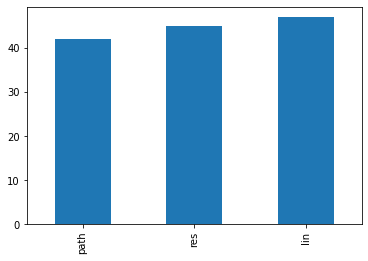
\includegraphics[width=6.5cm]{graph4.png}
\centering
\caption{A graph showing the accuracy of BERT, using 3 different semantic similarity measures (path, res, and lin).}
\end{figure}

As seen from the graph, there is over a 5\% difference in the accuracy when using different measures of semantic similarity. Path similarity gives us an accuracy of 42.06\%, and lin similarity gives an accuracy of 47.68\%. From this, we can assume that more investigation into techniques for comparing between predictions and options for answers will give us a higher overall accuracy. A suggestion for doing this would be with the use of a paraphrase identifier. A simple, one or two layer neural network that compares two sentences to see if they are paraphrases (i.e. to see if they have the same meaning) would be more accurate than just checking the semantic similarity of two words, and could show an even greater increase in accuracy.

Additionally, the accuracy of the system could be increased by fine-tuning the BERT model. BERT is specially designed so that an additional layer of transformers can be added to optimise the model for a specific task. We forked code from a public GitHub repository [see apendix 3] and made some slight alterations to accept our training data. Our system showed no significant increase in accuracy after being fine-tuned. This is most likely due to the fact that BERT is already trained as a masked language model, so our fine tuning does not have much impact on the output from the model, especially since we are limited by batch size, due to the power of the machine we are using to perform our research.

\section{Conclusion and Future Research Direction}
We have produced some good results in our experiments, increasing the accuracy of our system from a 20\% baseline, up to 47.68\% accuracy using a not-fine-tuned BERT masked language model. With more time to experiment with various systems and investigate alternatives, we may be able to increase this accuracy further.

With more time for research, we would create the neural n-gram variant discussed in section 3.3. We expect this model to have an accuracy higher than that of the trigram we constructed, at a reduced memory size, though we don't expect it to do as well as the pre-trained BERT model. The system sacrifices the ordering of the words in exchange for a wider context window which can look at a full sentence, and it would be more lenient when considering unknown words (due to smoothing), hopefully resulting in an increase in accuracy.

\newpage

\section{References}
https://www.microsoft.com/en-us/research/wp-content/uploads/2016/02/MSR\_SCCD.pdf
https://aclanthology.org/D13-1143.pdf
https://www.mdpi.com/2076-3417/10/4/1340
hopfield initial paper
https://link.springer.com/article/10.1007/s11023-020-09548-1
https://arxiv.org/abs/1810.04805v2

\section{Appendix}
\textbf{[1]} Link to Google Colab for code access. (see appendix 2 for GitHub link, and appendix 3 for raw code) https://colab.research.google.com/drive/17c6\_O0zERoGVoR78jPdmxHlYXXgexIm9?usp=sharing

\textbf{[2]} Link to GitHub for code access 
https://github.com/JamieBali/MRSCC

\textbf{[3]} GitHub link for BERT Fine-Tuning 
https://github.com/theartificialguy/NLP-with-Deep-Learning/blob/master/BERT/Fine\%20Tune\%20BERT/fine\_tuning\_bert\_with\_MLM.ipynb

\end{document}
